\label{sec:evaluation}
We evaluate the quality of our three topic models (LDA, SVD, and NMF) with three
experiments.  We focus first on evaluating aggregate coherence methods for a complete
topic model and consider the differences between each model as we learn an
increasing number of topics.  Secondly, we compare coherence scores to previous
semantic evaluations.  Lastly, we use the learned topics in a classification
task and evaluate whether or not coherent topics are equally informative when
discriminating between documents.

For all our experiments, we trained our models on 92,600 New York Times articles
from 2003 \cite{nytcorpus}.  For all articles, we removed stop words and any
words occurring less than 200 times in the corpus, which left 35,836 unique
tokens.  All documents were tokenized with OpenNLP's
MaxEnt\footnote{http://incubator.apache.org/opennlp/} tokenizer.  For the UCI
measure, we compute the PMI between words using a 20 word sliding window passed
over the WaCkypedia corpus \cite{baroni09wacky}.  In all experiments, we compute
the coherence with the top 10 words from each topic that had the highest weight,
in terms of LDA and NMF this corresponds with a high probability of the term
describing the topic but for SVD there is no clear semantic interpretation.

\subsection{Aggregate methods for topic coherence}

\begin{figure*}[h!t!b!]
  \centering
  \subfloat[UMass]{\label{fig:mean-umassNoSmooth}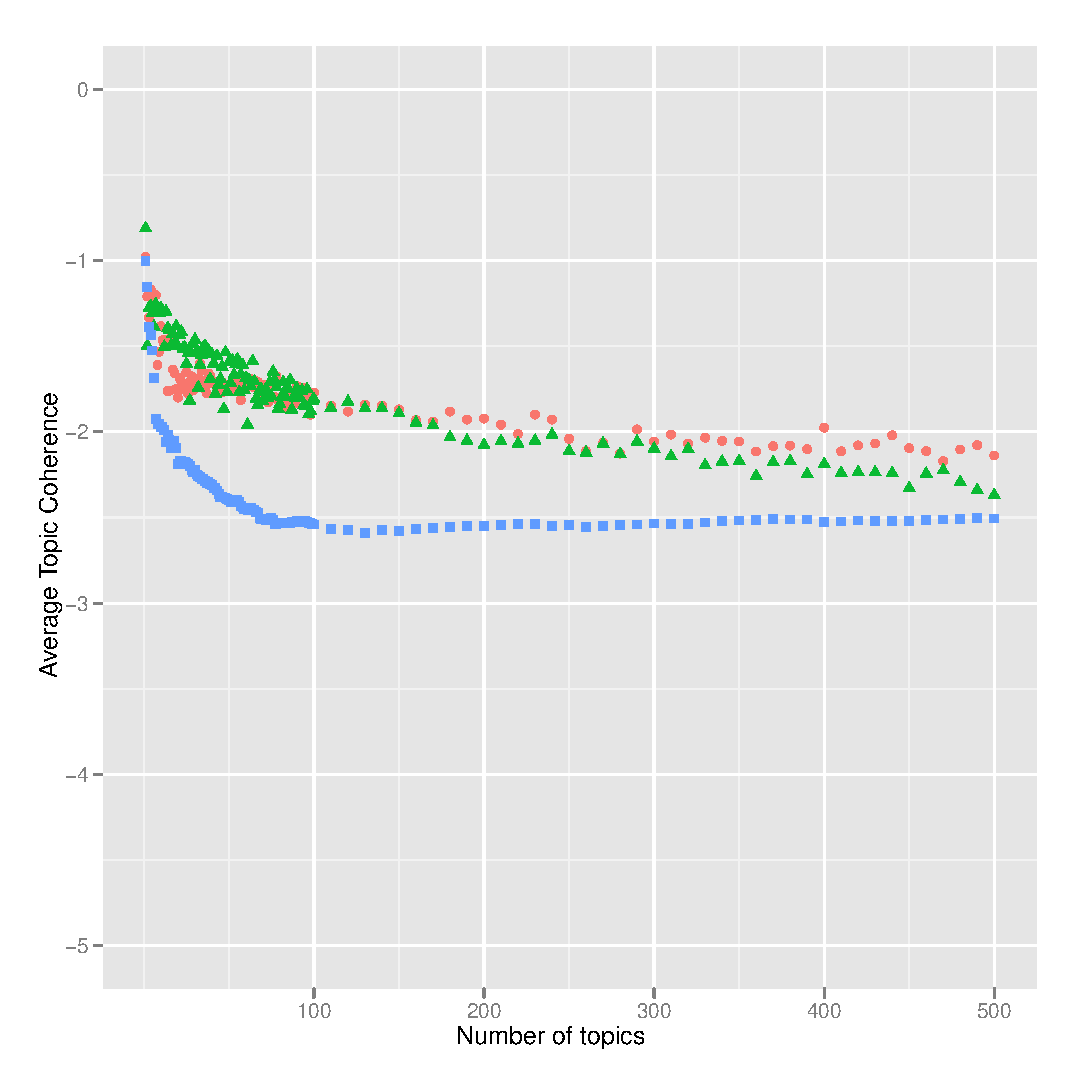
\includegraphics[width=.50\textwidth,height=.35\textwidth]{plots/mean-umassNoSmoothing.eps}}
  \subfloat[UCI]{\label{fig:mean-uciNoSmooth}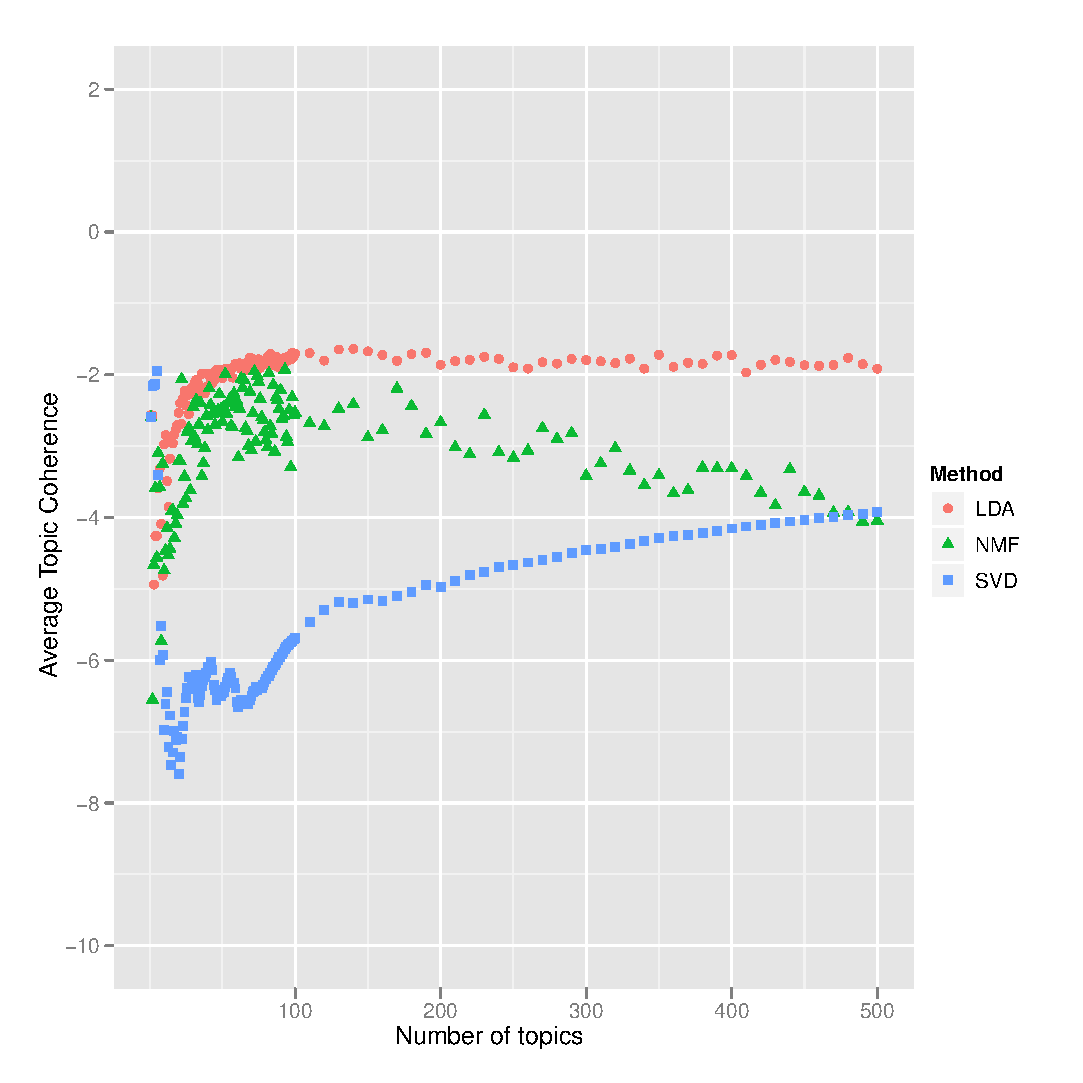
\includegraphics[width=.50\textwidth,height=.35\textwidth]{plots/mean-uciNoSmoothing.eps}}
  \caption{Average Topic Coherence with $\epsilon=10^{-12}$}
  \label{fig:mean-smoothing}
\end{figure*}

\begin{figure*}[h!t!b!]
  \centering
  \subfloat[UMass]{\label{fig:10mean-umassNoSmooth}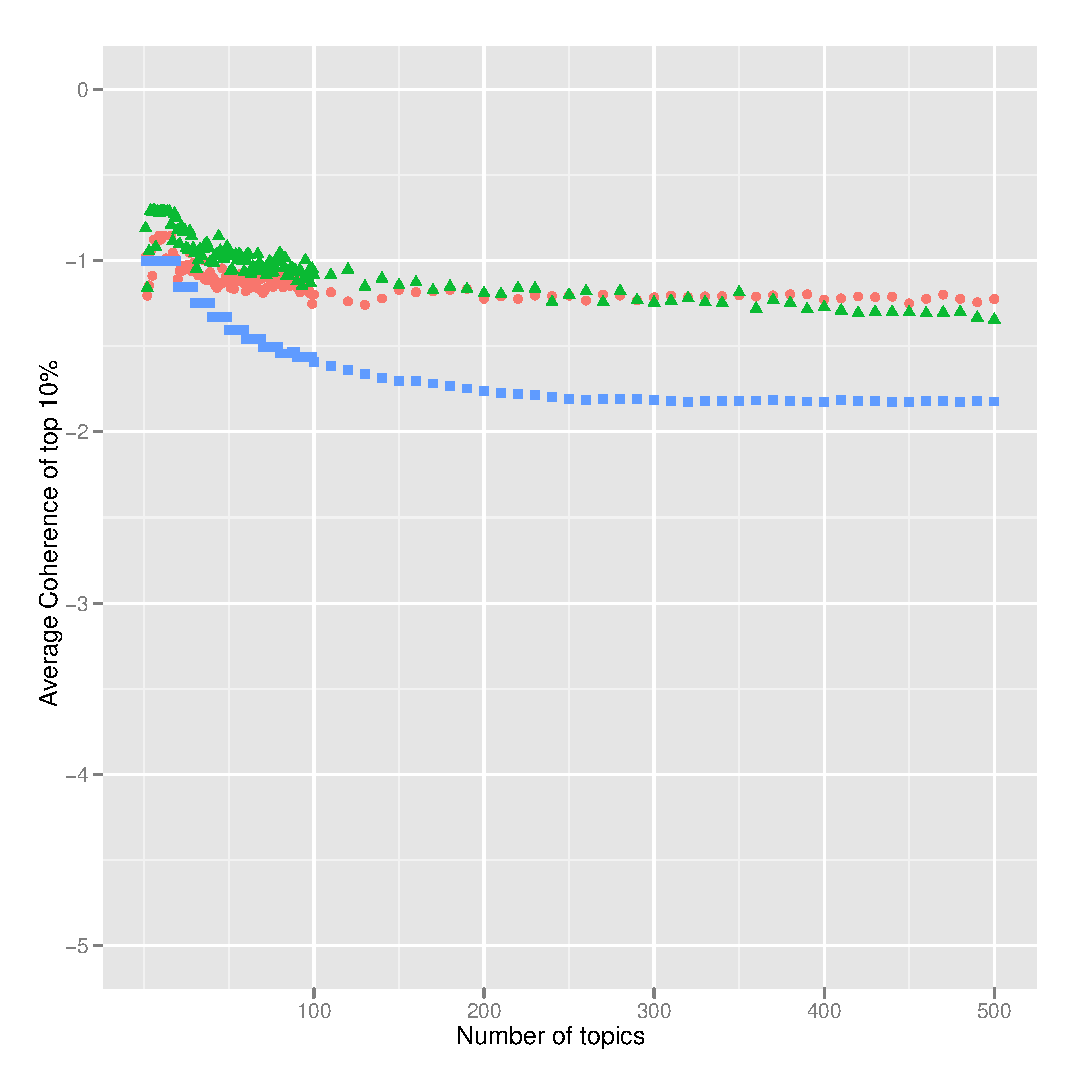
\includegraphics[width=.50\textwidth,height=.35\textwidth]{plots/10mean-umassNoSmoothing.eps}}
  \subfloat[UCI]{\label{fig:10mean-uciNoSmooth}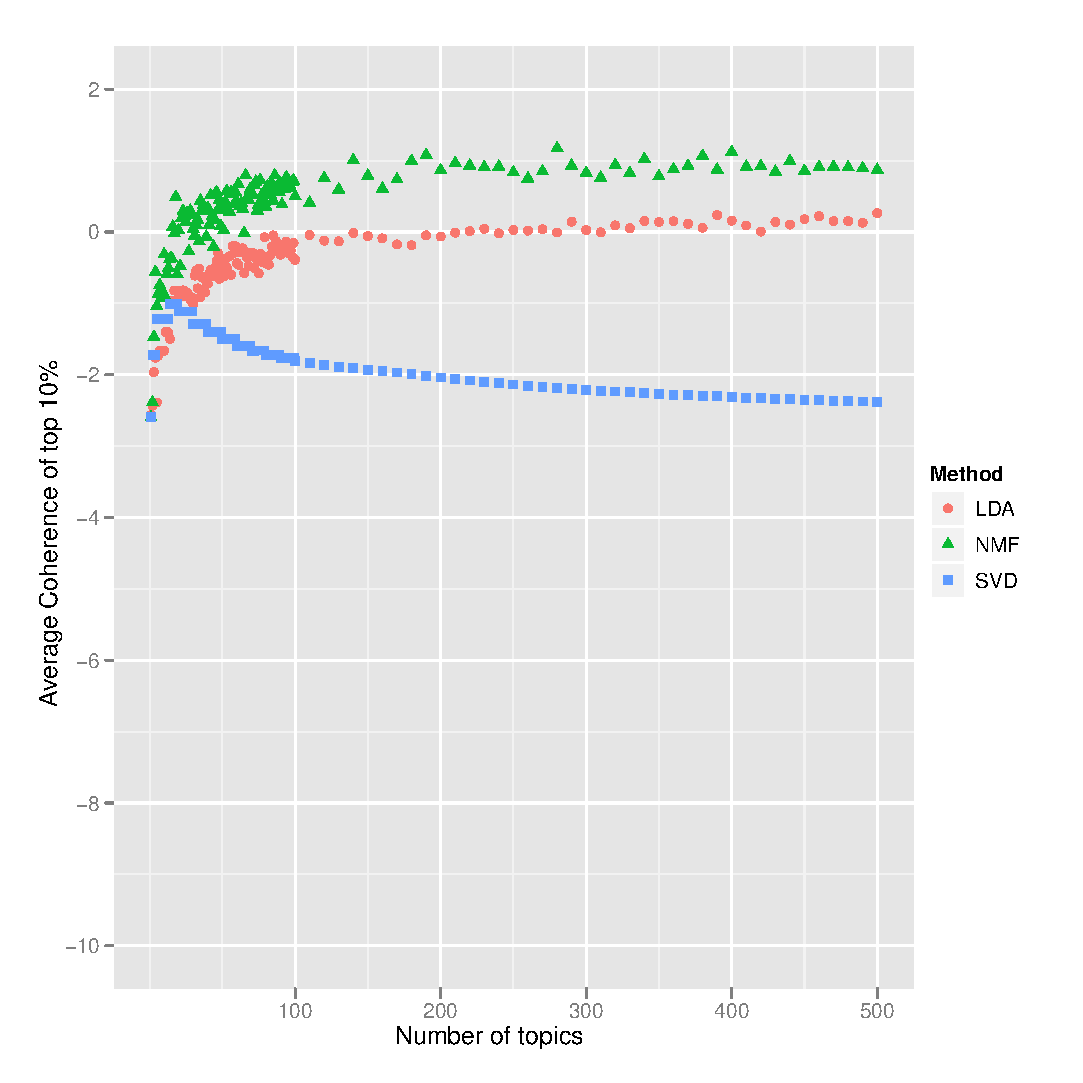
\includegraphics[width=.50\textwidth,height=.35\textwidth]{plots/10mean-uciNoSmoothing.eps}}
  \caption{Average Topic Coherence of the top 10\% topics with $\epsilon=10^{-12}$}
  \label{fig:10mean-smoothing}
\end{figure*}

Before we can compare topic models, we require an aggregate
measure that represents the quality of a complete model, 
rather than individual topics.  We consider two aggregates methods:
(1) the average coherence of all topics and
(2) the entropy of the coherence for all topics.  
The average coherence provides a quick summarization of a model's quality
whereas the entropy provides an alternate summarization that differentiates
between two interesting situations.  Since entropy measures the complexity of a
probability distribution, it can easily differentiate between uniform
distributions and multimodal, distributions.  This distinction is relevant when
users prefer to have roughly uniform topic quality instead of a wide gap between
high- and low-quality topics, or vice versa.  We compute the entropy by dropping
the $log$  and $\epsilon$ factor from each scoring function.

Figure \ref{fig:mean} shows the average coherence scores for each model as we
vary the number of topics.  These average scores indicate some simple
relationships between the models: LDA and NMF have approximately the same
performance and both models are consistently better than SVD.  All of the models
quickly reach a stable average score at around 100 topics.  This initially
suggests that learning more topics neither increases or decreases the quality of
the model, but Figure \ref{fig:entropy} indicates otherwise.  While the entropy
for the UMass score stays stable for all models, NMF produces erratic entropy
results under the UCI score as we learn more topics.  As entropy is higher for
even distributions and lower for all other distributions, these results suggest
that the NMF is learning topics with drastically different levels of quality,
i.e. some with high quality and some with very low quality, but the average
coherence over all topics do not account for this.

\begin{comment}
\begin{figure*}[h!t!b!]
  \centering
  \subfloat[UMass]{\label{fig:ordered-umassNoSmooth}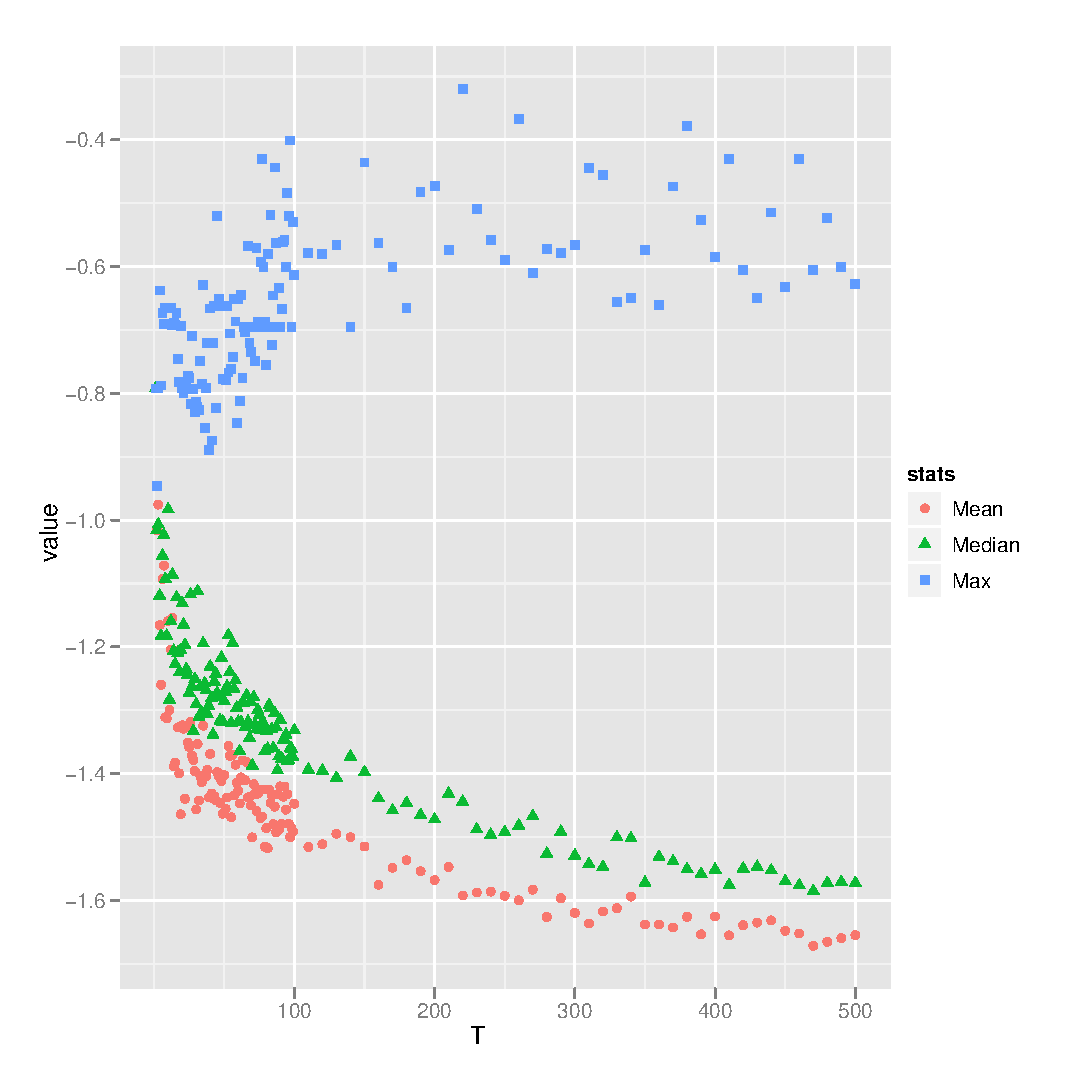
\includegraphics[width=.50\textwidth,height=.35\textwidth]{plots/lda-nmf-umass.eps}}
  \subfloat[UCI]{\label{fig:ordered-uciNoSmooth}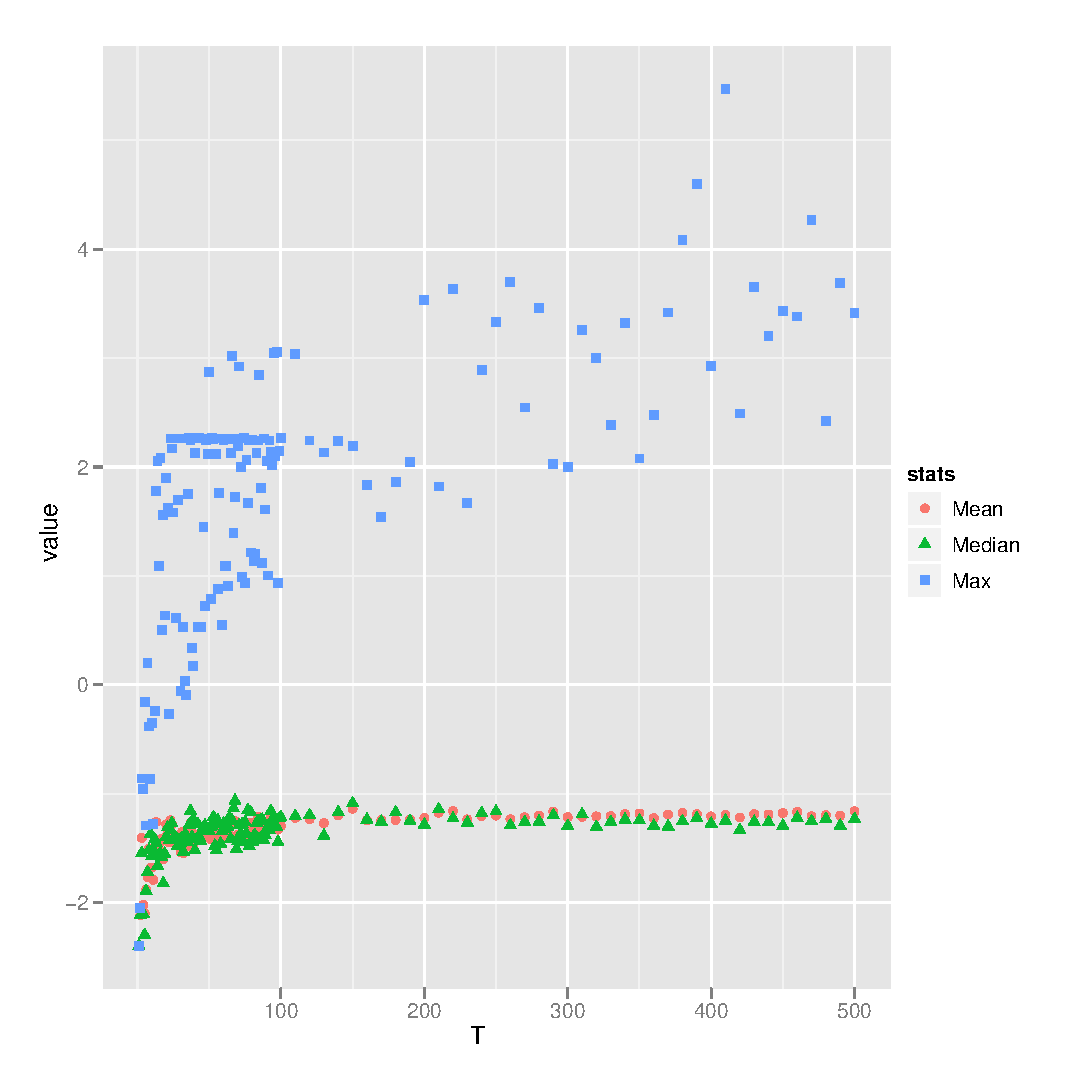
\includegraphics[width=.50\textwidth,height=.35\textwidth]{plots/lda-nmf-uci.eps}}
  \caption{Bipartite weights between LDA and NMF models using the Hungarian Algorithm}
  \label{fig:paired-weights}
\end{figure*}

\begin{figure*}[h!t!b!]
  \centering
  \subfloat[UMass]{\label{fig:ordered-umassNoSmooth}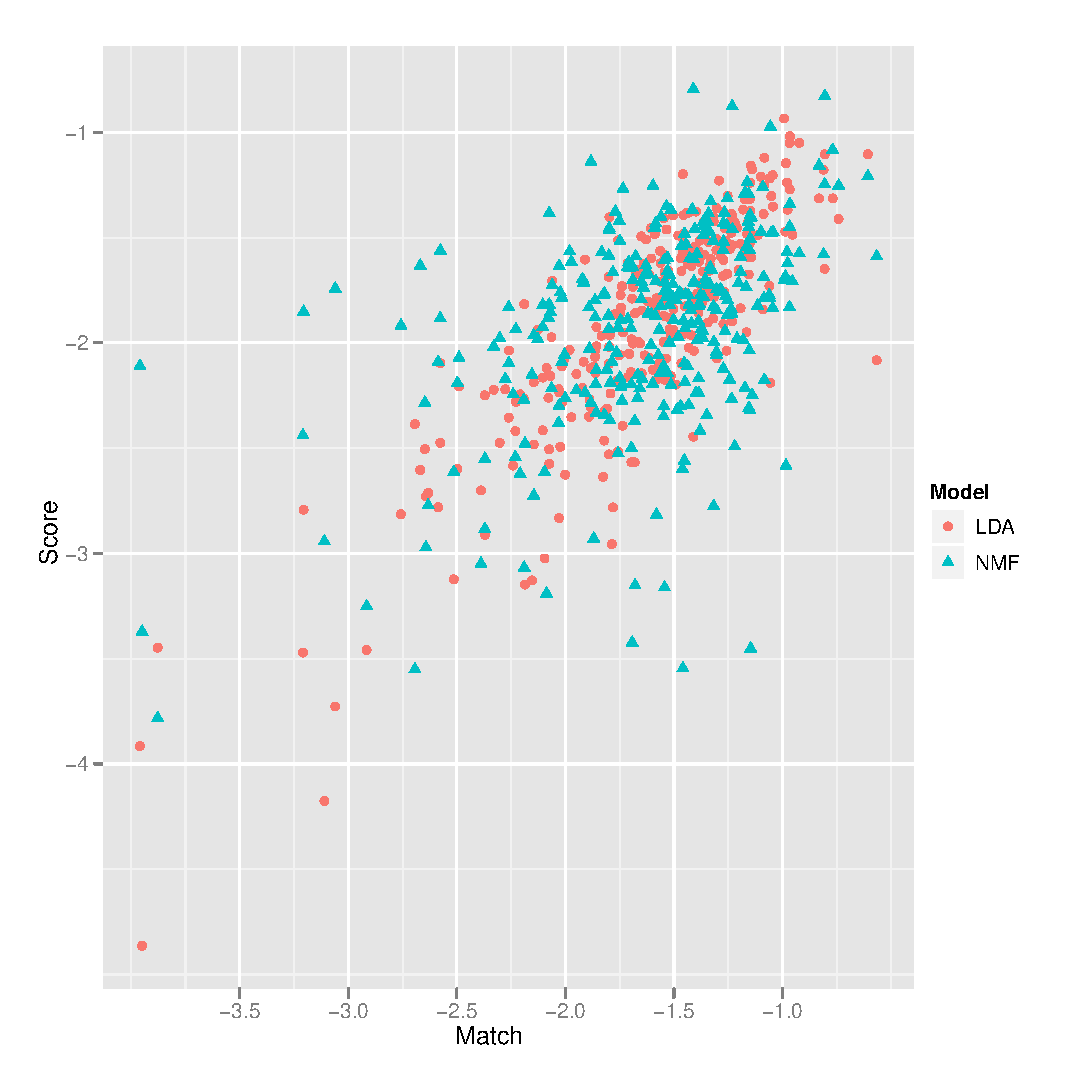
\includegraphics[width=.50\textwidth,height=.35\textwidth]{plots/lda-nmf-umass-300.eps}}
  \subfloat[UCI]{\label{fig:ordered-uciNoSmooth}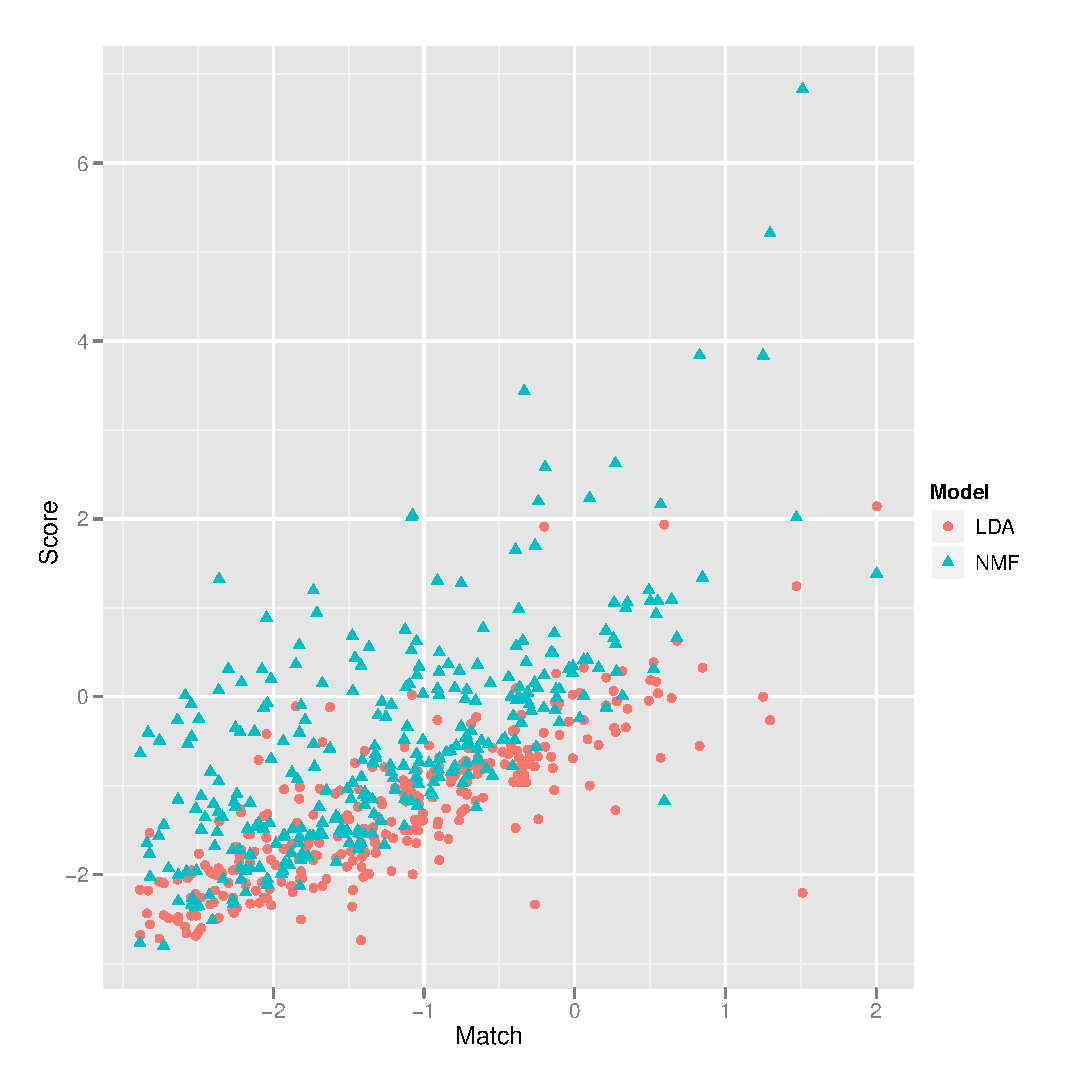
\includegraphics[width=.50\textwidth,height=.35\textwidth]{plots/lda-nmf-uci-300.eps}}
  \caption{Relation between bipartite weights and topic coherence scores for 300 topics}
  \label{fig:score-weight-300}
\end{figure*}
\end{comment}

\begin{figure*}[h!t!b!]
  \centering
  \subfloat[Rubenstein \&
  Goodenough]{\label{fig:rng-wordsim}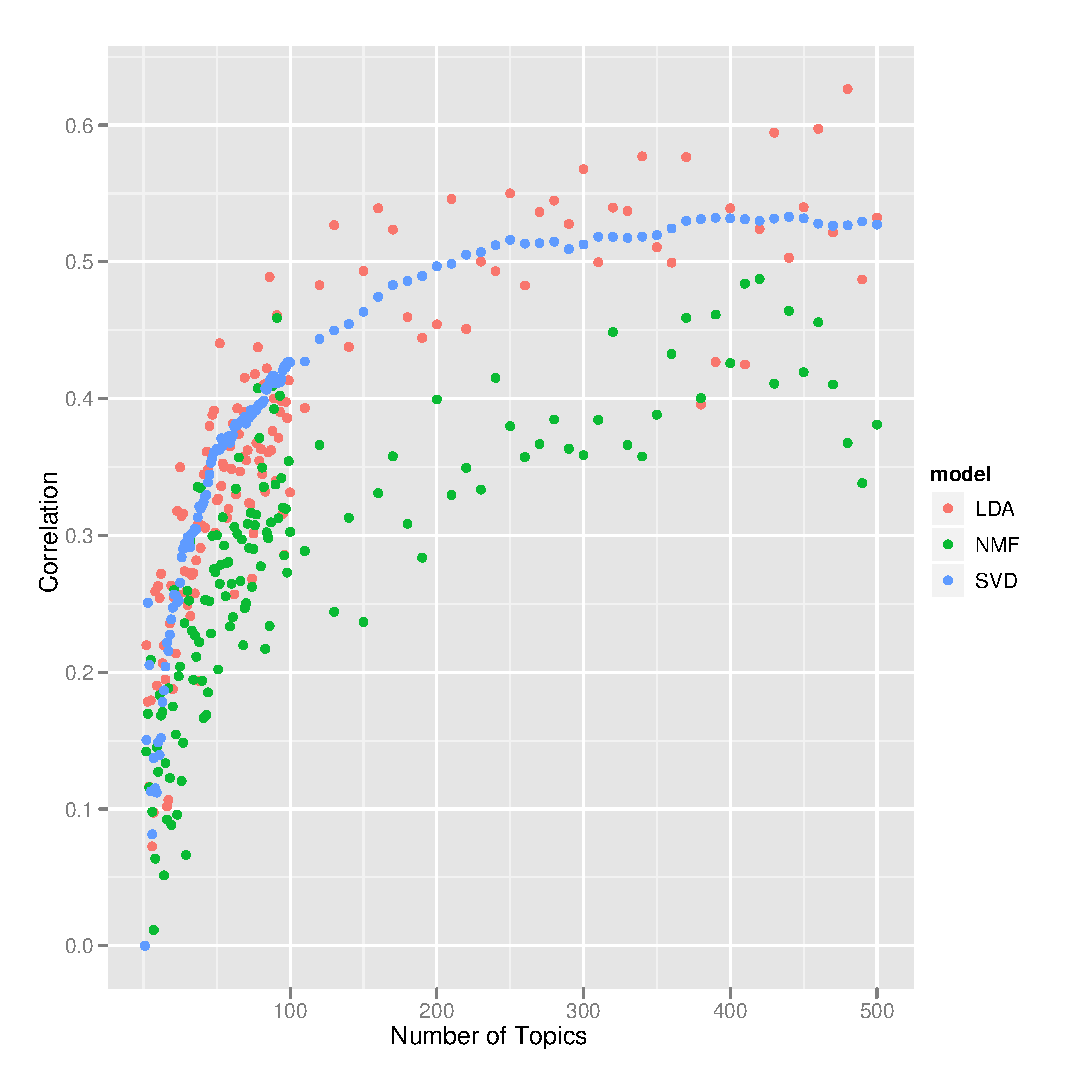
\includegraphics[width=.50\textwidth,height=.35\textwidth]{plots/rng_wordsim.eps}}
  \subfloat[Wordsim
  353/Finklestein~et.~al.]{\label{fig:353-wordsim}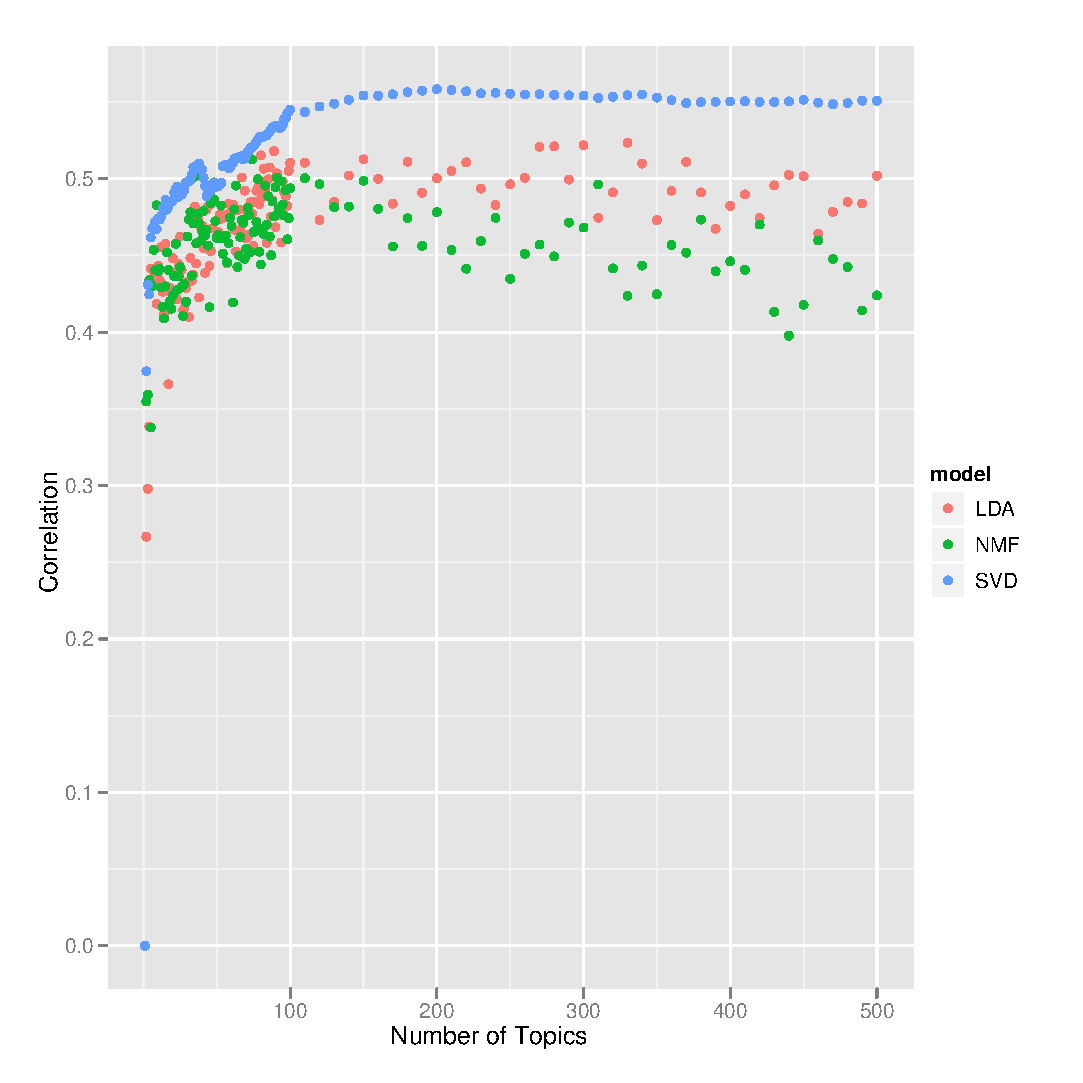
\includegraphics[width=.50\textwidth,height=.35\textwidth]{plots/353_wordsim.eps}}
  \caption{Word Similarity Evaluations for each model}
  \label{fig:wordsim}
\end{figure*}

\begin{figure}[h!t!b!]
  \centering
  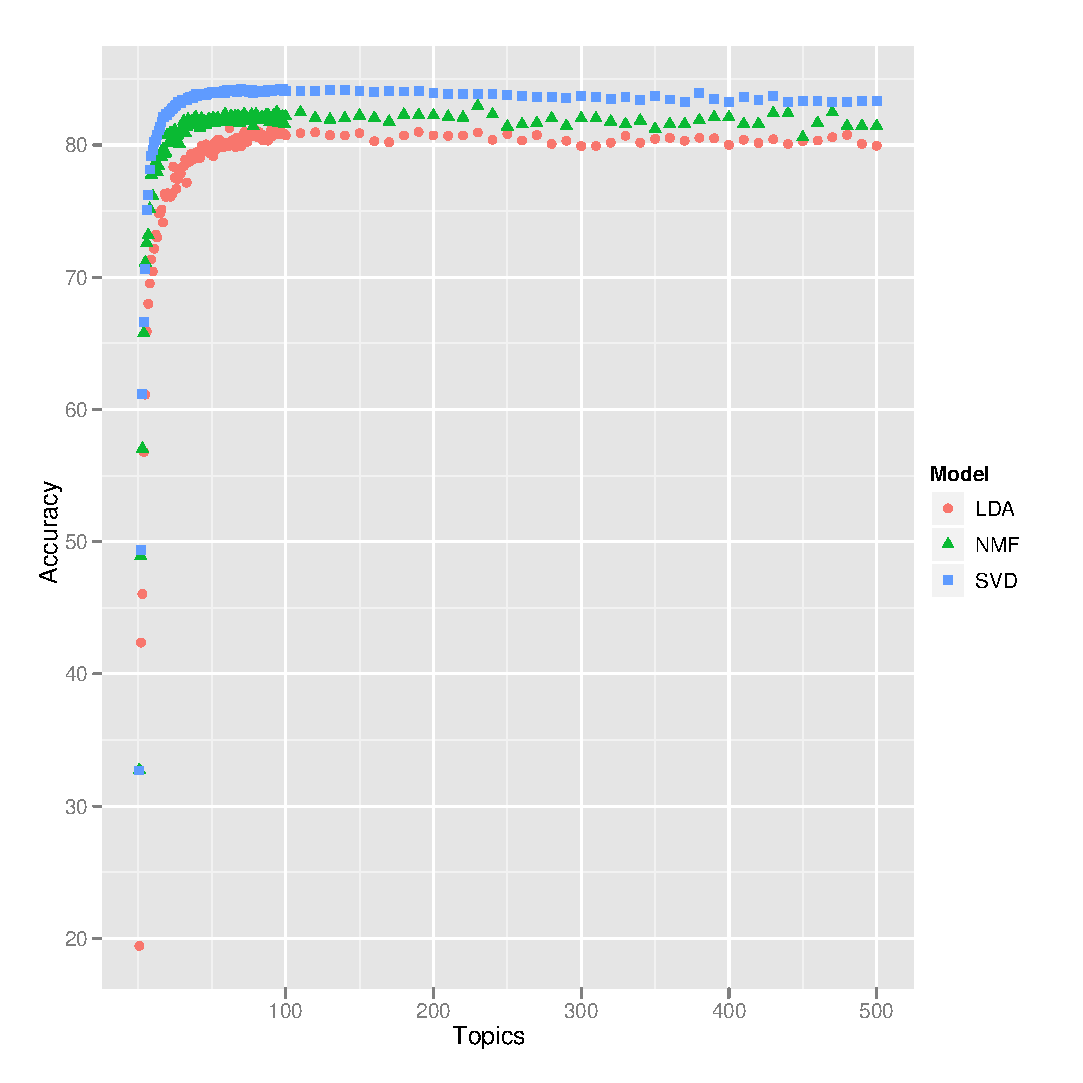
\includegraphics[width=.50\textwidth,height=.35\textwidth]{plots/avatar_classifier.eps}
  \caption{Classification accuracy for each model}
  \label{fig:predict}
\end{figure}

Low quality topics may be composed of highly unrelated words that
can't be fit into another topic, and in this case, our smoothing
factor, $\epsilon$, may be artificially increasing the score for
unrelated words. Following the practice of the original use of these
metrics, in Figures~\ref{fig:mean} and \ref{fig:entropy} we set
$\epsilon = 1$. In Figure~\ref{fig:mean-smoothing}, we consider
$\epsilon = 10^{-12}$, which should significantly reduce the score for
completely unrelated words. Here, we see a significant change in the
performance of NMF, the average coherence decreases dramatically as we
learn more topics. Similarly, performance of SVD drops dramatically
and well below the other models. In figure \ref{fig:10mean-smoothing}
we lastly compute the average coherence using only the top 10\% most
coherence topics with $\epsilon = 10^{-12}$. Here, NMF again performs
on par with LDA. With the top 10\% topics still having a high average
coherence but the full set of topics having a low coherence, NMF
appears to be learning more low quality topics once it's learned the
first 100 topics, whereas LDA learns fewer low quality topics in
general.

\begin{comment}
\begin{figure*}
  \centering
  \subfloat[UMass]{\label{fig:ordered-umass}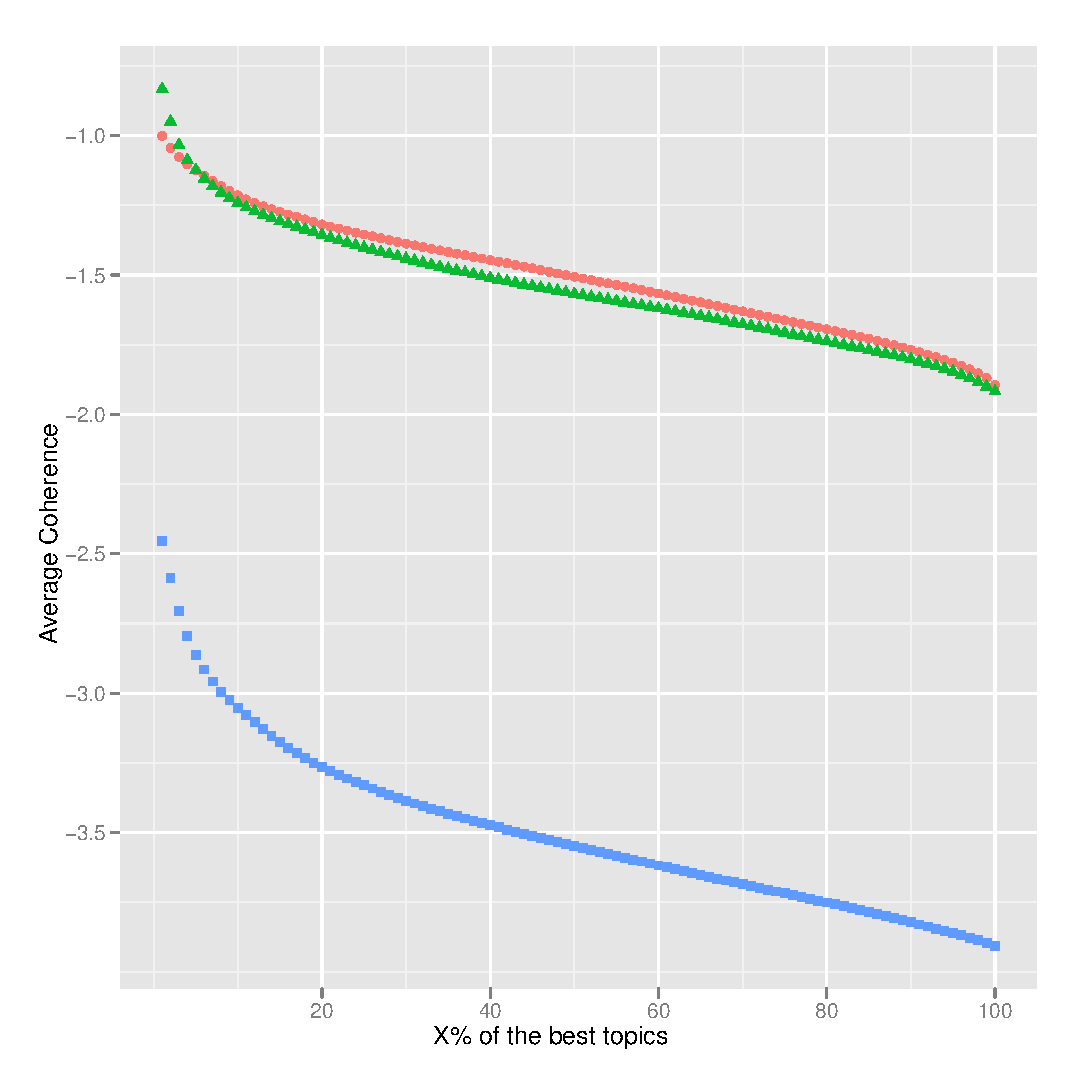
\includegraphics[width=.50\textwidth,height=.35\textwidth]{plots/ordered_300_umass.eps}}
  \subfloat[UCI]{\label{fig:ordered-uci}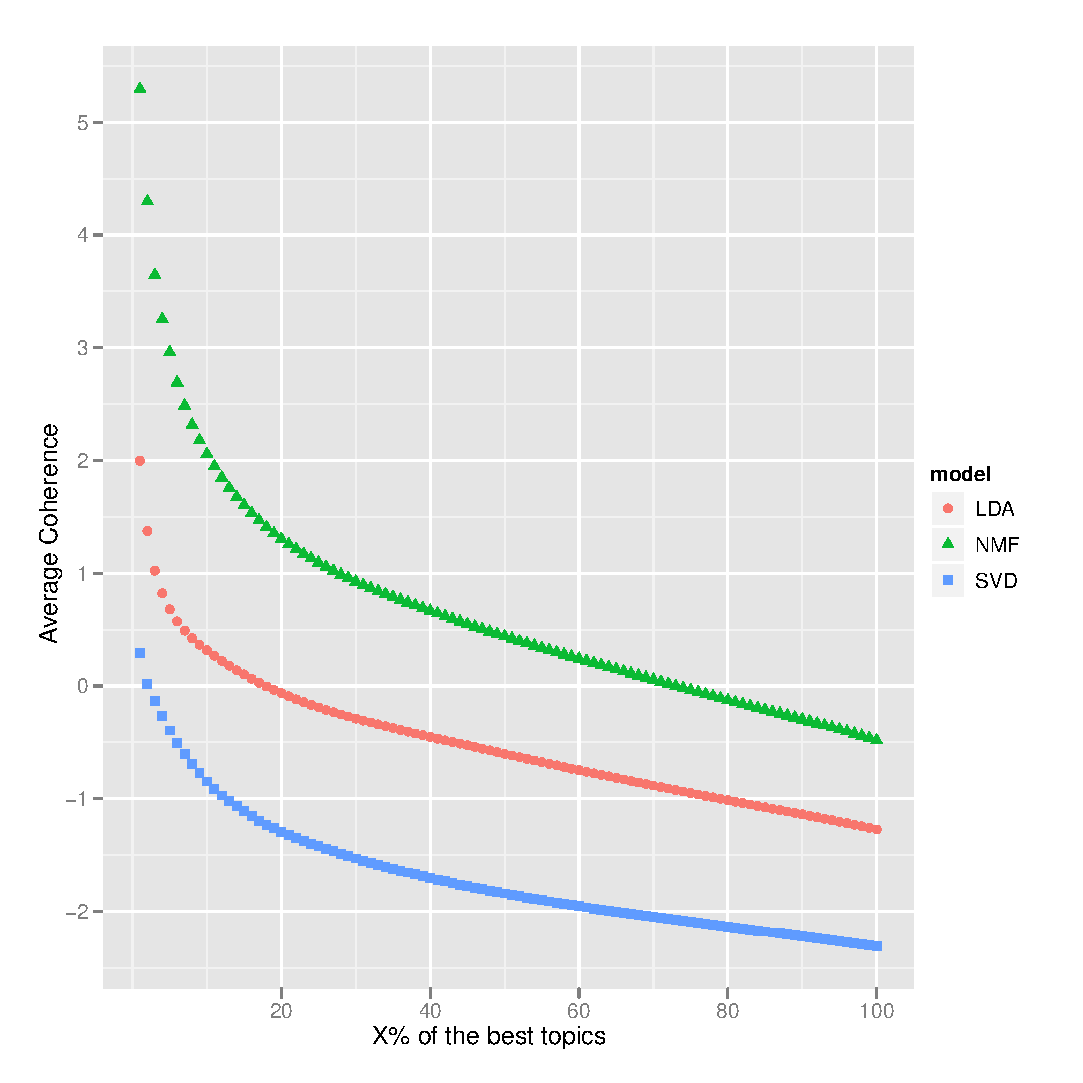
\includegraphics[width=.50\textwidth,height=.35\textwidth]{plots/ordered_300_uci.eps}}
  \caption{Topic Coherence for the top X\% topics out of 300 topics}
  \label{fig:top10avg}
\end{figure*}

\begin{figure*}
  \centering
  \subfloat[UMass]{\label{fig:ordered-umassNoSmooth}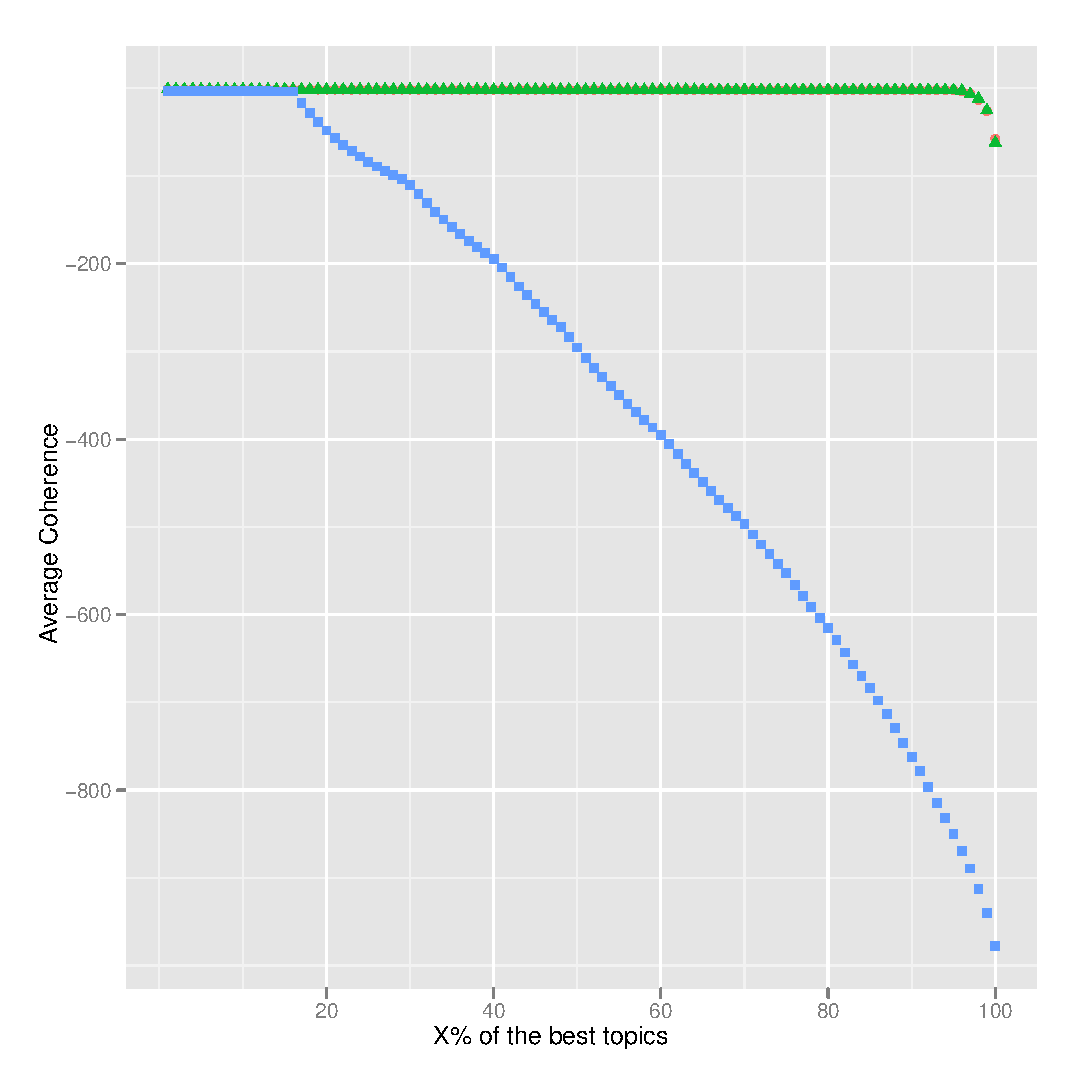
\includegraphics[width=.50\textwidth,height=.35\textwidth]{plots/ordered_300_umassNoSmoothing.eps}}
  \subfloat[UCI]{\label{fig:ordered-uciNoSmooth}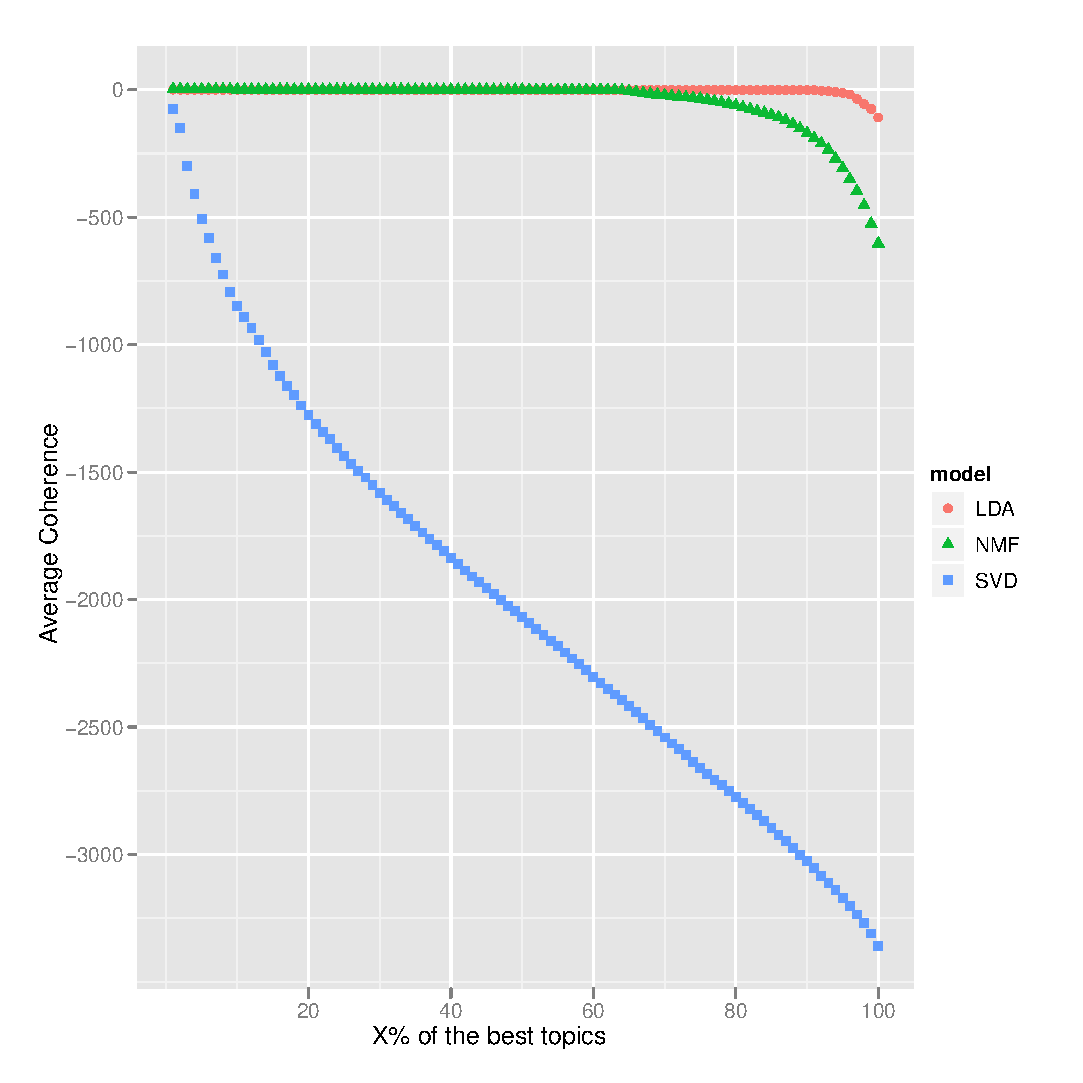
\includegraphics[width=.50\textwidth,height=.35\textwidth]{plots/ordered_300_uciNoSmoothing.eps}}
  \caption{Topic Coherence for the top X\% topics out of 300 topics with $\epsilon=10^{-12}$}
  \label{fig:top10avg}
\end{figure*}

\begin{figure}
  \centering
  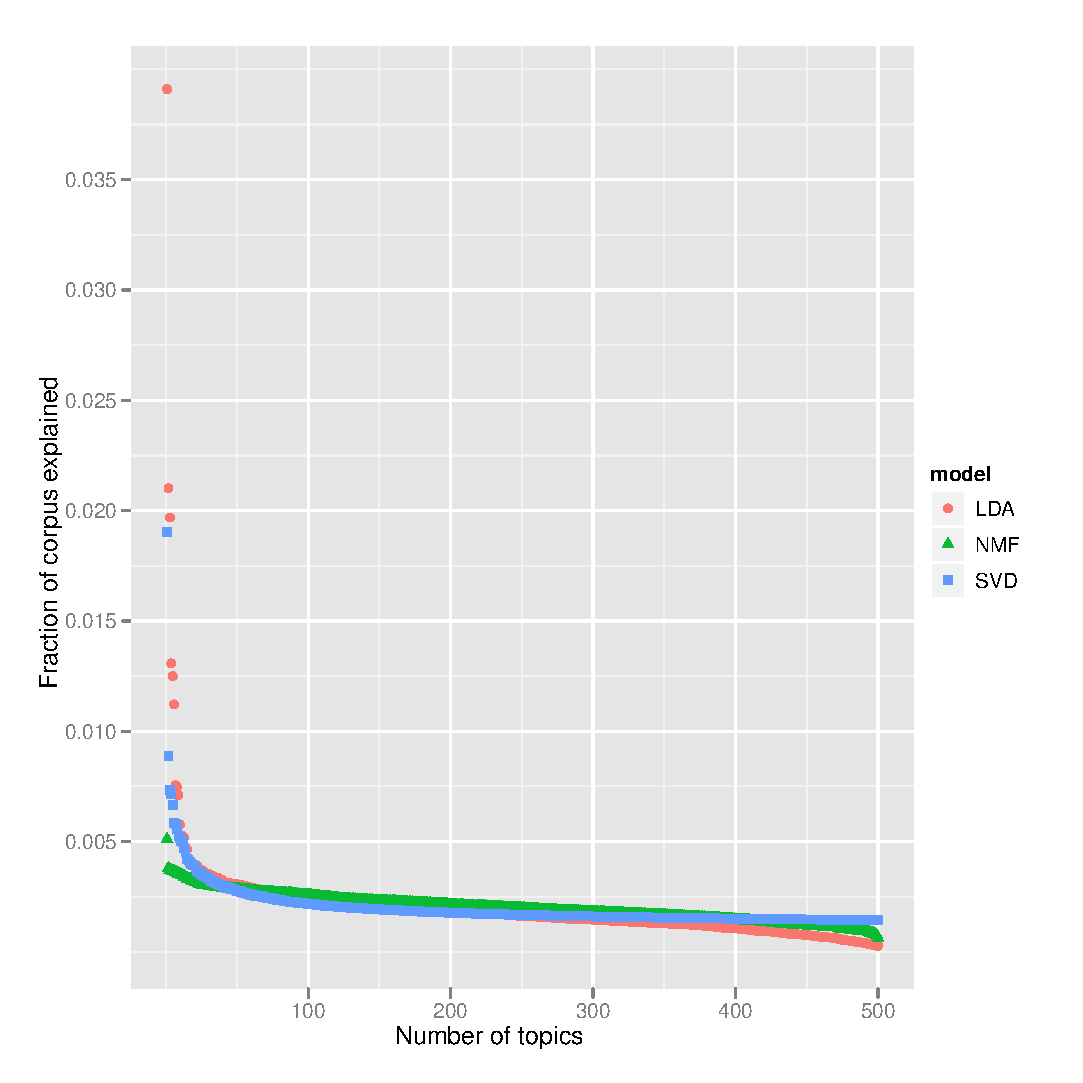
\includegraphics[width=.50\textwidth,height=.35\textwidth]{plots/model_topic_probs.eps}
  \caption{The inherent strength of each topic in descending order}
  \label{fig:topicProbs}
\end{figure}
\end{comment}

\begin{comment}
\subsection{Matching Topics}

In the previous experiment, LDA and NMF regularly produced the most coherent
topics, thus.  With such similar scores, we wish to know whether or not the two
models are learning similar topics.  For example, are the best 10 topics from
LDA equivalent to the best 10 topics from NMF?  To address this possibility, we
find the coherence between a pair of topics, $V$ and $Z$ with the following
measure:

$$pairCoherence(V, Z) = \sum_{v_i \in V, z_j \in Z} score(v_i, z_i)$$

Now, we can compare the coherence, or relatedness, between topics
between two models by first comparing the $pairCoherence$ between all topic
combinations between two models and then finding the best matching topics with
the Hungarian Algorithm, which finds an optimal bipartite matching.  If two
models are learning the same topics, we would expect the best matching to be
high, otherwise we can be confidence that the two models are learning unique
sets of topics, and thus users could potentially use both models.

\begin{table}[h]
\footnotesize
\center
\begin{tabular}{|c|c|p{1.75in}|}
\hline
Quality & Model & Topic Terms \\
\hline
\multirow{2}{*}{Best}
& LDA & wine wines bottle grapes made winery cabernet grape pinot red \\
& NMF & tannins chardonnay sauvignon wine 2000 vintages tasting merlot cabernet wines \\
\hline
\multirow{2}{*}{Worst}
& LDA & page front paper article news writer 24 16 28 read \\
& NMF & lists designations 3 7 serials boy 2 witchcraft 8 paperbacks \\
\hline
\end{tabular}
\label{tab:match-words}
\caption{The top 10 words from the best and worst matching topics from LDA and
NMF}
\end{table}

We show the $pairCoherence$ scores first in Figure
\ref{fig:paired-weights} using both coherence scoring methods.  This plots the
best, the average, and the median matching scores between LDA and NMF as we
learn a variable number of topics.  The maximum scores show that both LDA and
NMF are learning at least one highly similar topic.  Consider the best paired
topics from LDA and NMF when using the UCI measure in table
\ref{tab:match-words}.  Here, both models clearly learned a topic about wines
and wine making.  Also as expected, the two least connected topics have no
noticeable connection.  Furthermore, the medians and averages indicate that the
rest of the topics are also mutually coherent.  

We last consider the relation between $pairCoherence$ and the topic coherence
for the topics from each model.  Figure \ref{fig:score-weight-300} makes this
comparison directly for each model.  Under both measures the $pairCoherence$ and
topic coherence show a clear but somewhat weak correlation, as the
$pairCoherence$ increases, so does the topic coherence, especially for the best
matched topics.  

\end{comment}
\subsection{Word Similarity Tasks}

\begin{figure*}[h!t!b!]
  \centering
  \subfloat[UMass]{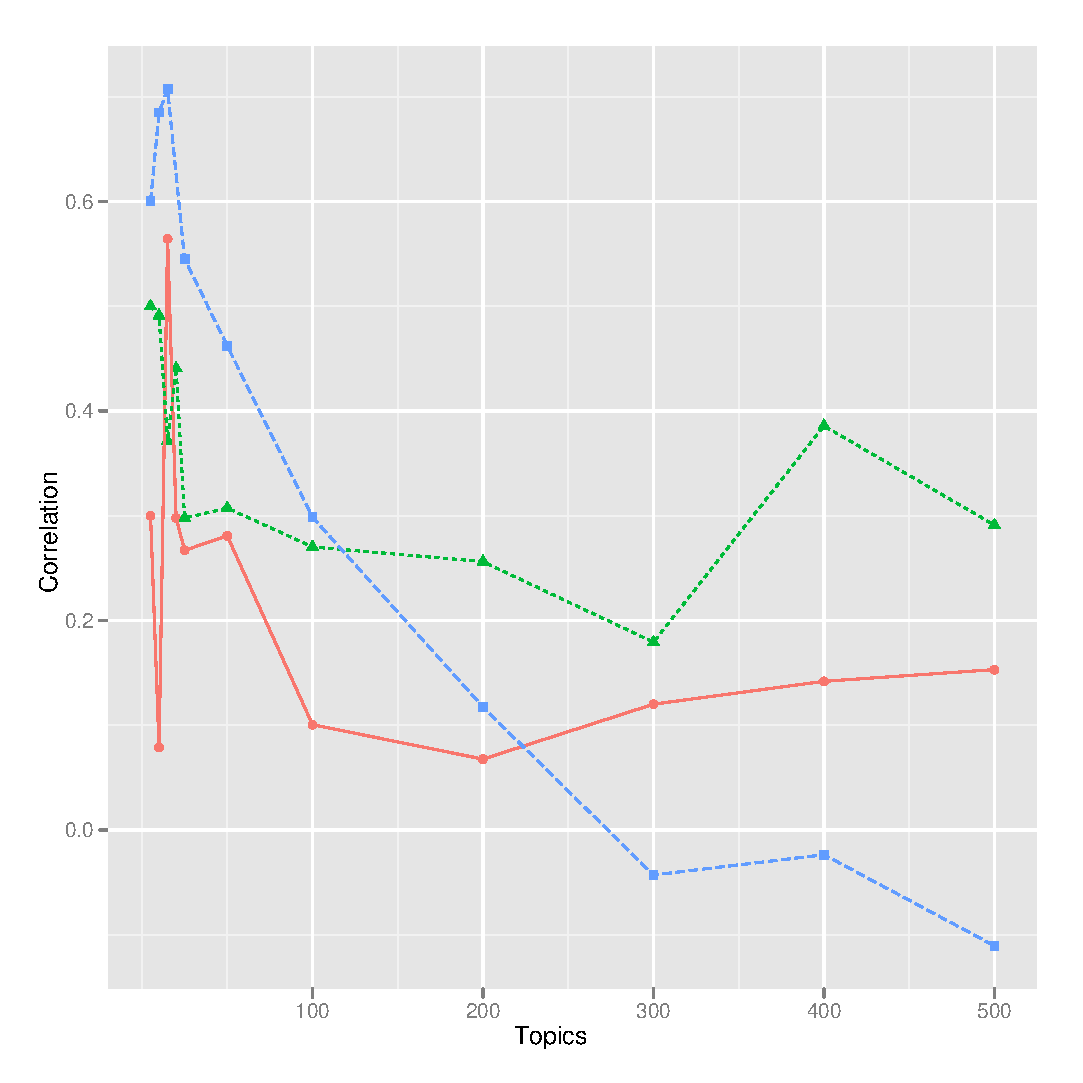
\includegraphics[width=.50\textwidth,height=.35\textwidth]{plots/umassNoSmoothing-ranks.eps}}
  \subfloat[UCI]{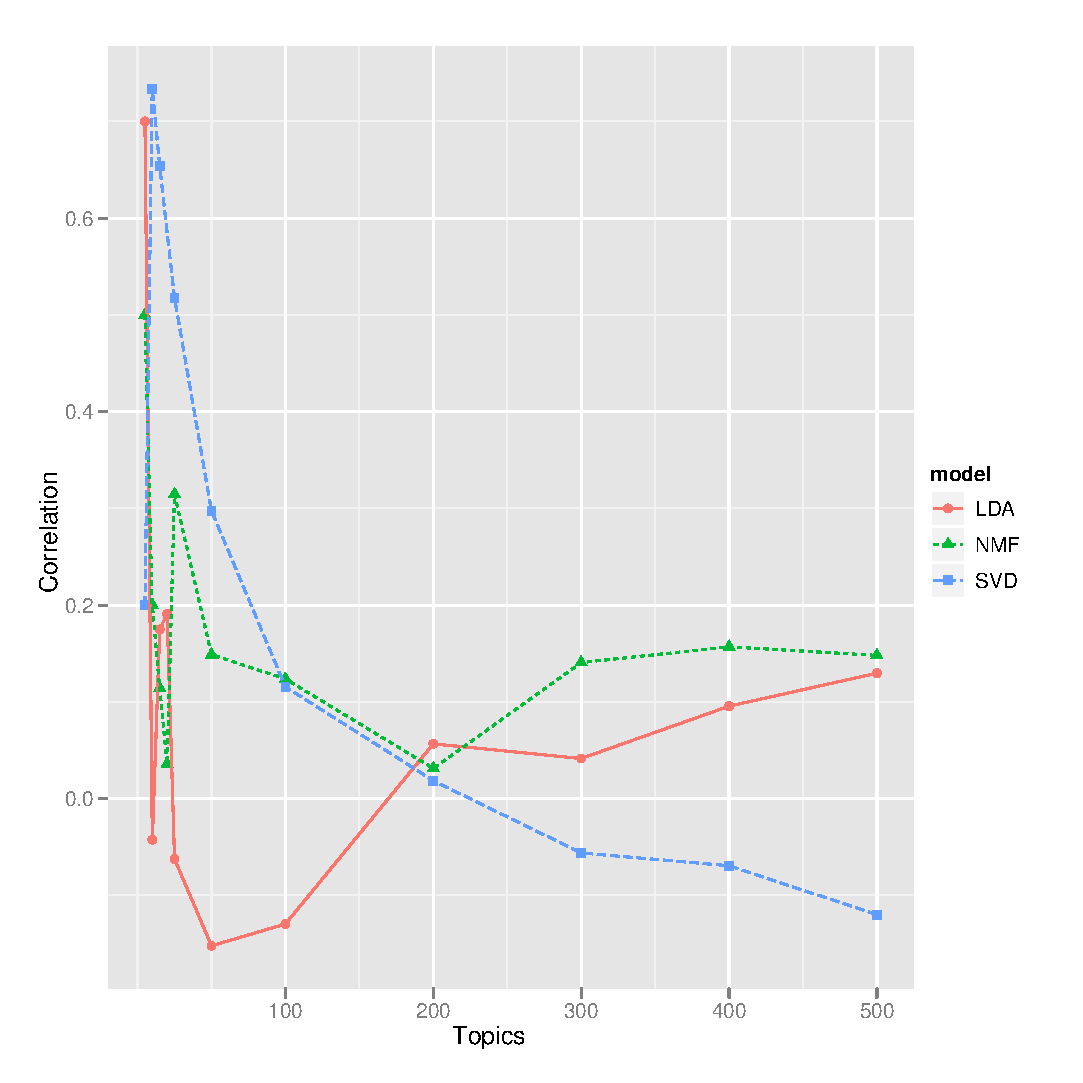
\includegraphics[width=.50\textwidth,height=.35\textwidth]{plots/uciNoSmoothing-ranks.eps}}
  \caption{Correlation between topic coherence and topic ranking in
  classification}
  \label{fig:topic-ranks}
\end{figure*}

\begin{figure*}[h!t!b!]
  \centering
  \subfloat[UMass]{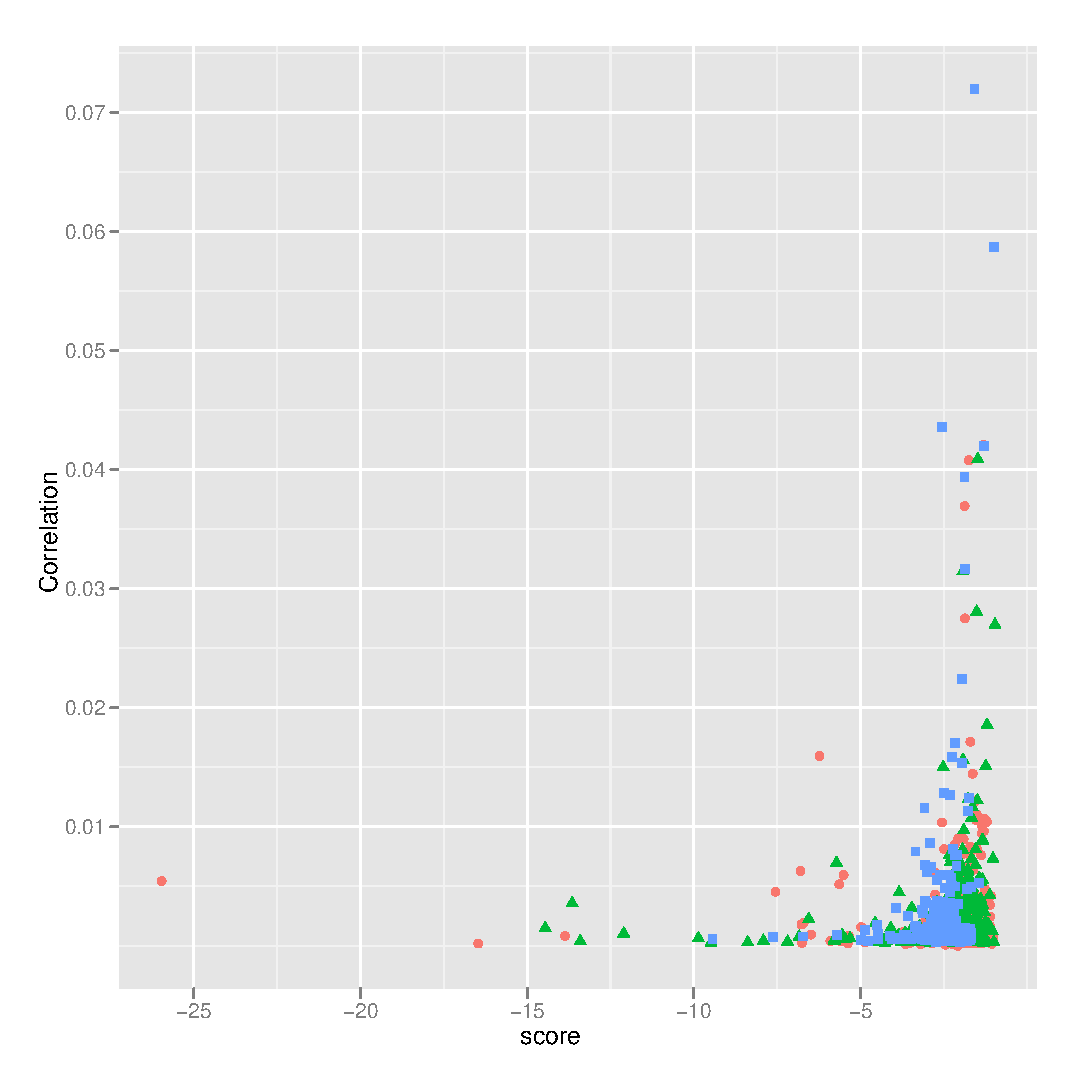
\includegraphics[width=.50\textwidth,height=.35\textwidth]{plots/umassNoSmoothing-rank-500.eps}}
  \subfloat[UCI]{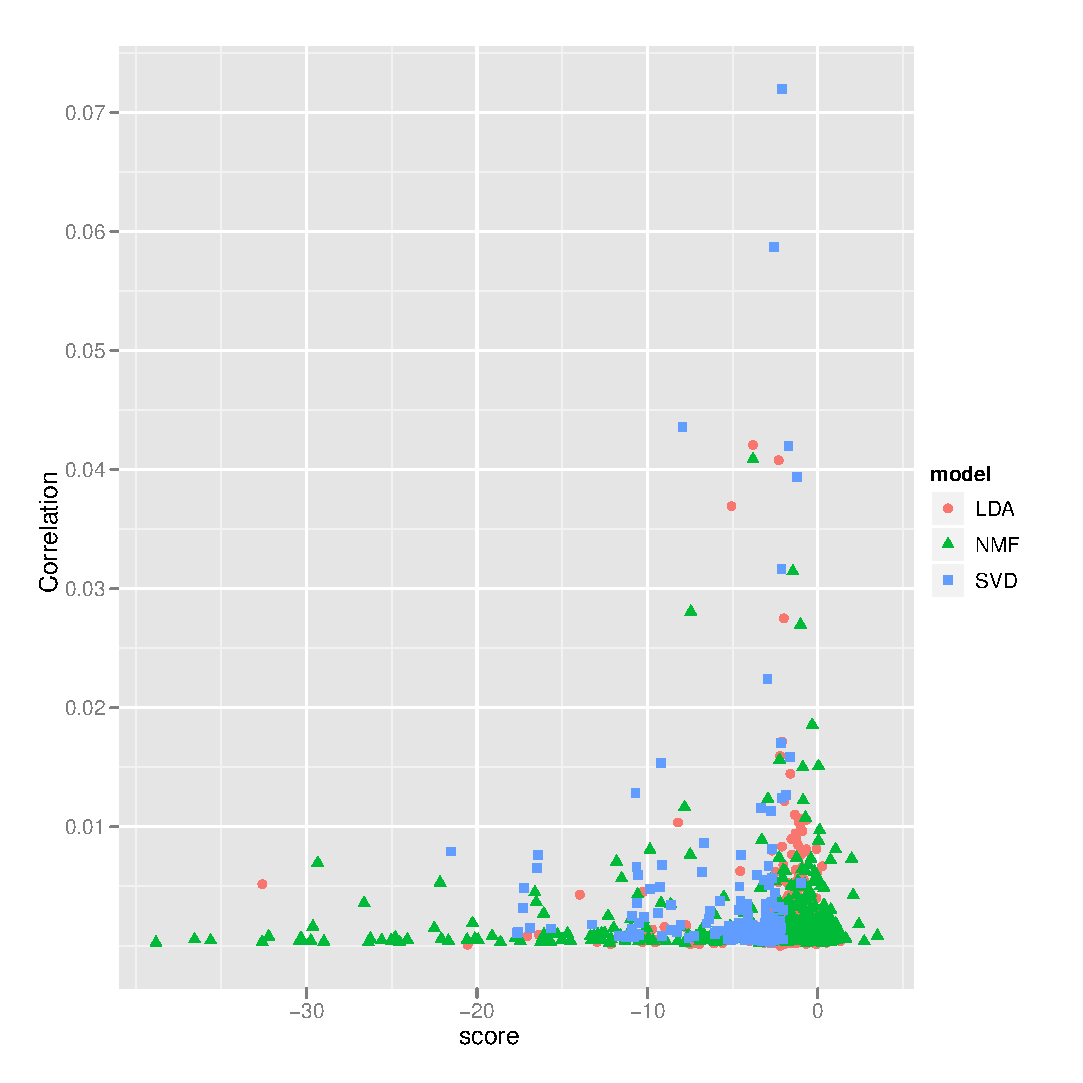
\includegraphics[width=.50\textwidth,height=.35\textwidth]{plots/uciNoSmoothing-rank-500.eps}}
  \caption{Comparison between topic coherence and topic rank with 500 topics}
  \label{fig:ranks500}
\end{figure*}

The initial evaluations for each coherence measure asked human judges to
directly evaluate topics \cite{newman10uci,mimno11umass}.  We expand upon this
comparison to human judgments by considering word similarity tasks that have
often been used to evaluate distributional semantic spaces
\cite{jurgens10sspace}.  Here, we use the learned topics as generalized
semantics describing our knowledge about words.  If a model's topics generalize
the knowledge accurately, we would expect similar words, such as ``cat'' and
``dog'', to be represented with a similar set of topics.  Rather than evaluating
individual topics, this similarity task considers the knowledge within the
entire set of topics, the topics act as more compact representation for the
known words in a corpus.

We use the \newcite{rubenstein65wordsim} and \newcite{finkelstein02relatedness}
word similarity tasks.  In each task, human judges were asked to evaluate the
similarity or relatedness between different sets of word pairs.   Fifty-One
Evaluators for the \newcite{rubenstein65wordsim} dataset were given 65 pairs of
words and asked to rate their similarity on a scale from 0 to 4, where a higher
score indicates a more similar word pair.  \newcite{finkelstein02relatedness}
broadens the word similarity evaluation and asked 13 to 16 different subjects
to rate 353 word pairs on a scale from 0 to 10 based on their relatedness, where
relatedness includes similarity and other semantic relations.  We can evaluate
each topic model by computing the cosine similarity between each pair of words
in the evaluate set and then compare the model's ratings to the human ratings by
ranked correlation.  A high correlation signifies that the topics closely model
human judgments.  

Figure \ref{fig:wordsim} displays the results.  SVD and LDA both surpass NMF on
the Rubenstein \& Goodenough test while SVD is clearly the best model on the
Finklestein et. al test.  While our first experiment showed that SVD was the
worst model in terms of topic coherence scores, this experiment indicates that
SVD provides an accurate, stable, and reliable approximation to human judgements
of similarity and relatedness between word pairs in comparison to other topic
models.

\subsection{Coherence versus Classification}

For our final experiment, we examine the relationship between topic
coherence and classification accuracy for each topic model.  We suspect that
highly coherent topics, and coherent topic models, will perform better for
classification.  We address this question by performing a document
classification task using the topic representations of documents as input features
and examine the relationship between topic coherence and the usefulness of the
corresponding feature for classification.

We trained each topic model with all 92,600 New York Times articles as before.
We use the section labels provided for each article as class labels, where each
label indicates the on-line section(s) under which the article was published and
should thus be related to the topics contained in each article.  To reduce the
noise in our data set we narrow down the articles to those that have only one
label and whose label is applied to at least 2000 documents.   This results in
57,696 articles with label distributions listed in Table \ref{tab:labels}.  We
then represent each document using columns in the topic by document matrix $H$
learned for each topic model.

\begin{table}[htbp]
  \centering
  \begin{tabular}{lr|lr}
    Label & Count & Label & Count \\ \hline
    New York and Region & 11219 &  U.S. & 3675	\\   
    Paid Death Notices & 11152 &   Arts & 3437	\\   
    Opinion & 8038 &               World & 3330	\\   
    Business & 7494 &              Style & 2137	\\   
    Sports & 7214 
  \end{tabular}
  \caption{Section label counts for New York Times articles used for
  classification}
  \label{tab:labels}
\end{table}

For each topic model trained on N topics, we performed stratified 10-fold
cross-validation on the 57,696 labeled articles. In each fold,
we build an automatically-sized bagged ensemble of unpruned CART-style decision
trees\cite{banfield07compareensemble} on 90\% of the
dataset\footnote{The precise choice of the classifier scheme matters
little, as long as it is accurate, speedy, and robust to label noise;
all of which is true of the choice here.}, use that ensemble
to assign labels to the other 10\%, and measure the accuracy of that assignment.
Figure \ref{fig:predict} shows the average classification accuracy over all ten
folds for each model.  Interestingly, SVD has slightly, but statistically
significantly, higher accuracy results than both NMF and LDA.  Furthermore,
performance quickly increases and plateaus with well under 50 topics.

Our bagged decision trees can also determine the importance of each feature
during classification.  We evaluate the strength of each topic during
classification by tracking the number of times each node in our decision trees
observe each topic, please see \cite{Caruana06miningcitizen} for more details.
Figure \ref{fig:ranks500} plot the relationship between this feature ranking and
the topic coherence for each topic when training LDA, SVD, and NMF on 500
topics.  Most topics for each model provide little classification information,
but SVD shows a much higher rank for several topics with a relatively higher
coherence score.  Interestingly, for all models, the most coherent topics are
not the most informative.  Figure \ref{fig:topic-ranks} plots a more compact
view of this same relationship: the Spearman rank correlation between
classification feature rank and topic coherence.  NMF shows the highest
correlation between rank and coherence, but none of the models show a high
correlation when using more than 100 topics.  SVD has the lowest
correlation, which is probably due to the model's overall low coherence yet high
classification accuracy.  

